\section{Topic Segmentation Evaluation}
\subsection{A Lack of Corpora}
    Large corpora of training data for conversation topic segmentation do not exist, especially within the context of conversations, which causes two issues:
    \begin{enumerate}
        \item We can not train a \textbf{supervised} \gls{model} to detect boundary changes such as in \cite{joty2013topic}.
        \item Our quantitative evaluation is not representative of all conversations that we analyse and uncertainties are quite high.
    \end{enumerate}

\subsection{Our Evaluation Methods \label{method: segmentation evaluation}}
    In contexts other than conversations, algorithms are evaluated on chapters of medical textbooks\cite{eisenstein2008bayesian, simon2013leveraging}. Section titles are removed from the text and the algorithm is evaluated by how similarly its predicted boundaries are to the original section boundaries. Unfortunately, no such data exists for conversations.

    \subsubsection{Quantitative Evaluation}
        To quantify segmentation techniques, we annotate a 4 conversation sections (each ca. 250 sentences) by hand. To do this, we read through a transcript and place a boundary indicator in the text where we believe the topic of the conversation has changed. We try to annotate a representative sample of transcripts, but as this is a very time consuming process and conversation structure varies a lot, uncertainties are high and results statistically less significant than desired. We annotate sections from the podcasts shown in Table \ref{table: hand annotated podcasts}. They were chosen because we believe them to represent different types of conversations and a wide range of topics.

        \newcolumntype{b}{X}
        \newcolumntype{s}{>{\hsize=.5\hsize}X}

       \begin{table}[h]
       \centering
            \begin{tabularx}{0.9\textwidth}{| s | b | s | }
            \hline
            \textbf{Podcast Title}       & \textbf{Episode Title}                       & \textbf{Description}      \\ \hline
            Joe Rogan Experience         & \#1470 Elon Musk                             & Casual Conversation       \\ \hline
            Making Sense with Sam Harris & \#190 --- How Should We Respond to Coronavirus & Expert Interview          \\ \hline
            143 Pixels                   & CaptLogun --- World of Warcraft Classic        & Expert Conversation       \\ \hline
            6 Drunk 1 Sober              & Too Drunk                                    & Casual Group Conversation \\ \hline
            \end{tabularx}
            \caption{Podcasts of which we annotate a small subsection for evaluation purposes.}
            \label{table: hand annotated podcasts}
        \end{table}

    \subsubsection{Metric}
    We use the WindowDiff measure\cite{pevzner2002critique}, $w_d$ to rate segmentation. It moves a window of size $\Delta u$ across the segmented text and penalises the algorithm whenever the number of segmentation boundaries within the window does not match the ``true" (i.e. human annotated) number of boundaries for that window. Thus, a lower $w_d$ is better. We choose $\Delta u$ to be half the size of average segments in the true segmentation as is typical in the literature\cite{purver2006unsupervised}\cite{eisenstein2008bayesian}.

    \subsubsection{Future Improvements}
    For future research, we propose the creation of a data set similar to the medical textbook but for conversations, based on YouTube transcriptions:
    The video sharing platform YouTube allows video creators to split their video into segments called ``chapters"\cite{YoutubeChapters}. Some content creators, such as podcast host and artificial intelligence researcher Lex Fridman\cite{LexFridmanYoutube}, use these chapters to label topics. We hypothesise that if videos of conversations were transcribed and annotated with their ``chapter" titles, they could be used as a training set and evaluation set for topic segmentation in conversation.


%\subsection{Utterance Embedding Clustering \label{method: utterance embedding clustering}}
%    \begin{figure}[t]
%        \centering
%        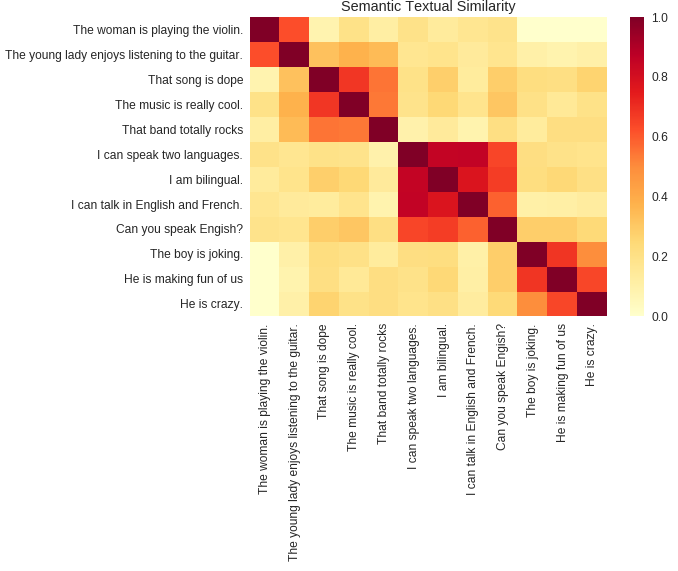
\includegraphics[width=0.8\textwidth]{sentence_similarity.png}
%        \caption{Using Google's universal sentence encoder, sentences are embedded and their similarity visualised. The colour of the field at (row, column) indicates the similarity between the sentence labels at (row, column). A darker colour indicates a stronger similarity.}
%        \label{fig:sentence similarity}
%    \end{figure}
%    Using \gls{utterance} embeddings, similar sentences can be clustered together, forming topics. A visual example showing sentence similarity is shown in Fig. \ref{fig:sentence similarity}.
%    Going through the transcript, once the cluster to which a sentence is assigned changes, a topic boundary is set. This theoretically allows for topic segmentation.
%
%    \subsubsection{Minimum Cut Graph Based \label{method: minimum cut}}
%
%        Firstly we evaluate the minimum cut based clustering method detailed in Sec. \ref{fig: graph seg} for conversations, in which all \glspl{utterance} above some threshold similarity are clustered. The key limitation within the context of conversation is that certain \glspl{utterance} appear within all topics. Consider the following sample of \glspl{utterance}:
%        \begin{table}[h]
%            \begin{tabular}{l|l}
%            $u_1$     & \textit{Rock music is the best!}                        \\
%            $u_2$     & \textit{Yeah man, rock is the best!}                    \\
%            \dots      &                                                         \\
%            $u_i$     & \textit{Lord of the Rings is the best movie ever made.} \\
%            $u_{i+1}$ & \textit{Yeah dude, Lord of the Rings really is the best.}              \\
%            \end{tabular}
%        \end{table}
%
%        Even though $u_1$ and $u_{i}$ correctly do not connect, $u_1$ connects to $u_2$, $u_{i}$ connects to $u_{i+1}$ and critically, $u_2$ connects to $u_{i+1}$. This last connection is made because the sentences are similar, in fact everything \textit{except for the topic} matches between these \glspl{utterance}. In conversation, sentences like $u_2$ and $u_{i+1}$ are abundant - leading to one giant connected component, which is a cluster that contains a large fraction of all nodes. We attempted to fine-tune the cutoff similarity, but either (almost) no sentences end up connected or all of them do.
%        From testing the method, we thus qualitatively identify two issues:
%        \begin{enumerate}
%            \item Sentences in conversation often carry little meaning, particularly those only acknowledge/agree with previous \glspl{utterance}. These acknowledgements act as bridges between clusters.
%            \item The minimum cut clustering method amplifies this because one \gls{utterance} acting as a bridge suffices to connect two clusters.
%        \end{enumerate}
%
%        The first issue is the key problem with using \gls{utterance} embeddings. While the minimum cut method is particularly vulnerable, other clustering methods also suffer from it.
%
%    \subsubsection{Other Clustering Methods}
%        Since the cutoff-based approach lead to issues, we try the following clustering methods in an attempt to minimize the vulnerability to falsely merged clusters:
%        \begin{itemize}
%            \item k-means clustering, in which the algorithm tries to separate samples in k groups of equal variance.
%            \item DBSCAN clustering, in which clusters are viewed as areas of high density separated by areas of low density.
%            \item Agglomerative clustering, in which a hierarchy of clusters is formed by assigning each \gls{utterance} its own cluster and then repeatedly merging the most similar clusters.
%        \end{itemize}
%        All three clustering methods were implemented using the python library scikit-learn\cite{scikit-learn}. These clustering methods qualitatively perform better than the minimum cut method, but each suffer from new issues. In k-means, imposing the number of topics $k$ is difficult as it varies heavily from conversation to conversation. In DBSCAN clustering, which requires neither a cutoff nor a number of topics, if data points are not inherently clustered (i.e. separated by areas of low density), the algorithm fails. This occured for a significant fraction of \glspl{utterance}. The most promising algorithm for clustering was the agglomerative clustering method, in which some topics could be clearly identified, but qualitative results were too poor to warrant further development and quantitative evaluation.
%
%    \subsubsection{Limitations}
%        No matter the clustering method, using sentence \glspl{embedding} is ineffective when analysing conversation topics. Some words in sentences don't contribute to the meaning act as unwanted bridges to other topics, but they can also \textit{dilute} the embedding. Consider the \glspl{utterance}
%
%
%        \begin{table}[h]
%            \begin{tabular}{l|l}
%            $u_1$     & \textit{Do you have any pets?}                    \\
%            $u_2$     & \textit{We had a light brown cat as a family pet when I was younger, but I don't now.}                        \\
%            \end{tabular}
%        \end{table}
%
%        Both \glspl{utterance} are about pets, but because the question and answer share almost no other words, and because the answer is very long, the sentences are deemed dissimilar by the \gls{model}. %TODO: actually get the sim value
%
%
%        % Put this as limitation in TopicRank
%        Another issue is that \glspl{keyphrase} are often not repeated but still understood as the topic. Consider the following \glspl{utterance}:
%
%        \begin{table}[h]
%            \begin{tabular}{l|l}
%            $u_1$     & \textit{Do you have any pets?}                    \\
%            $u_2$     & \textit{Yeah I've got a cat.}                        \\
%            \end{tabular}
%        \end{table}
%
%        The word ``pet" is not repeated  but from the context of the conversation it is clear that the topic is still ``pets".
%
%        The issue with the \gls{utterance} \gls{embedding} approach can be succinctly summarised as the following: \Glspl{Utterances} are more than just their topics. While the similarity of \glspl{utterances} is correlated with the similarity of the topics in which they lie, they are not equivalent. To make a more effective algorithm, the words representing topics must be first extracted.
%
%\subsection{Latent Dirichlet Allocation - BayesSeg \label{method: LDA}}
%    \begin{table}[]
%    \centering
%    \begin{tabular}{lllll}
%    \hline
%    \textbf{Topic 1}   & \textbf{Topic 2}    & \textbf{Topic 3}   & \textbf{Topic 4} & \textbf{Topic 5}  \\ \hline
%    technology   & models        & speakers     & wouldn't   & v\_a\_d     \\
%    u\_m\_t\_s   & reverberation & overlaps     & you'd      & worse       \\
%    routing      & voicing       & alignment    & agree      & t\_i-digits \\
%    transmission & multi-band    & region       & matter     & baseline    \\
%    i\_p         & targets       & breath       & depends    & I\_d\_a     \\
%    mobile       & phonemes      & laugh        & open       & percent     \\
%    packet       & effects       & native       & others     & italian     \\
%    university   & echo          & backchannels & feeling    & improvement \\
%    concerning   & combining     & laughing     & term       & adaptation  \\
%    networking   & insertions    & marks        & opposed    & latency     \\ \hline
%    \end{tabular}
%    \caption{Sample topics from recorded meeting dialogues, extracted by the modified \gls{lda} algorithm by Purver et al.\cite{purver2006unsupervised}. Words within topics are vaguely related, such as topic 1 concerning networking technology, or topic 3 about \glspl{da}. However, a lot of words don't fit well together and are unlikely to represent a topic.}
%    \label{table: modified lda topics}
%    \end{table}
%
%    One method of segmentation that attempts to extract topic-words is the modified \gls{lda} method \textit{BayesSeg} proposed by Eisenstein et al.\cite{eisenstein2008bayesian} (see Sec. \ref{ssec: topic segmentation}). We choose this method over the similar method presented by Purver et al.\cite{purver2006unsupervised}, because BayesSeg can be applied to individual documents, while the segmentation method by Purver et al. requires a whole corpus of documents. We only received access to the Spotify podcast corpus shortly before the date of submission of this thesis and so could not evaluate said method. However, from the examples shown in the original paper by Purver et al.\cite{purver2006unsupervised}, shown in Table \ref{table: modified lda topics}, we believe the algorithms suffer from similar limitations.
%
%    BayesSeg achieves the WindowDiff penalty score
%    \begin{equation}
%     w_d = 0.39 \pm 0.06
%    \end{equation}
%    when segmenting our annotated transcripts. The uncertainty is quite high because we had to annotate evaluation data manually, which is a time-consuming process and was thus limited to 4 transcripts. This is a significantly worse score than the value reported for the ICSI-MRDA corpus, $w_d = 0.312$\cite{eisenstein2008bayesian}.
%
%    While the results could agree due to the high uncertainty, we hypothesise the following reason for this reduction in performance instead: \gls{lda} assumes that every word is generated by sampling a topic, which is a distribution over words. Every word is assumed to be part of a topic. In more robust media, such as scientific papers or newspaper articles, this may be an appropriate approximation: if the aim is to convey information efficiently, most words will be related to the topic that is discussed. To an extent, the formal business meetings in the ICSI-MRDA corpus still fit this description. In more casual conversations, however, a lot of words are not related to the topic discussed: they act as statements of politeness, as acknowledgements, to fill breaks of awkward silence or to be entertaining\cite{searle1965speech}. This could be an explanation for the worse performance of BayesSeg in casual conversations, and could be further investigated in future work by evaluating performance on more and less formal conversations.
%
%      We identify two further key issues with \gls{lda}-based methods for casual conversation and use examples from the segmentation \gls{model} by Purver et al., shown in Table \ref{table: modified lda topics}, to support them:
%    \begin{enumerate}
%        \item The lack of correlations captured by \gls{lda} as well as its inability to \gls{model} temporal topic evolution means that unrelated topics can be falsely grouped together. For example ``university" does not fit in Topic 1, and ``Italy" does not fit in Topic 5.
%        \item The generative assumption that every word describes a topic leads to topics of words that do not have coherent semantic meaning and appear frequently, reducing the effectiveness of segmentation. An example is Topic 4.
%    \end{enumerate}
%
%
%    %TODO: lda cant do correlations, if two different topics appear together, it sticks them together (t2, t3, t5 (italian)).
%    %Also: forcing every word to belong to topic leads to misfits e.g. "combining" in 2, "concerning" in 1,
%
%\subsection{TopicRank \label{method: topic rank}}
%
%Utterance embedding based methods (Sec. \ref{method: utterance embedding clustering}) as well as \gls{lda}-based methods (Sec. \ref{method: LDA} are somewhat ineffective for the segmentation of conversation in part because they assume that every word in every \gls{utterance} contributes to the topic of the conversation, which is false.
%TopicRank\cite{bougouin-etal-2013-topicrank} (see Sec. \ref{ssec: keyphrase extraction}) offers a promising alternative approach: it first extracts \glspl{keyphrase} that are likely to represent topics and discards the rest.
%
%\subsubsection{Evaluation}
%We use TopicRank on our hand-annotated transcripts and compare its selected topic-phrases against human-annotated topic-phrases. If a topic-phrase extracted by TopicRank, $t_{\text{TR}}$ has a similarity greater than
